\newpage
\section{Data} \label{sec:data}
We use data collected by the Consumer Expenditure Survey (CEX) that is administered by the Bureau of Labor Statistics. Additionally to the main questionnaire, the CEX added questions about the stimulus payments to their surveys conducted between June 2008 and March 2009 (\textbf{isthis correct time in dataset?}). The main advantage of the CEX is that it creates a unique representative sample that contains finely grained information on the type of goods households consume. While its main purpose is to serve as the benchmark to determine the goods basket used to measure inflation in the USA, it enables a detailed analysis on what households spent their rebate on. In the following, we briefly outline the stimulus program and describe the CEX data. 

\subsection{The 2008 Tax Stimulus Program} 
Due to the global financial crisis and the subsequent recession, the United States government passed the Economic Stimulus Act (ESA) in February 2008. With projected costs of more than 150 billion USD it was the largest relief program passed in the history of the USA. Next to the stimulus payments, which made up roughly two thirds of the program, the ESA also enacted other steps meant to provide economic relief such as enabling government owned entities (Fannie Mae and Freddie Mac) to buy up more mortgages. However, we only focus on the effects of the stimulus payments. \\
The rebate was paid out to any household that filed for income taxes (\textbf{unsure about the wording of 'to file for taxes'}) and reported a minimum annual income of 3,000 USD in 2007. Eligible households received their net tax liability as their rebate, however, the payment were bounded by a minimum of 300 and a maximum of 600 USD. For couples filing jointly the limits were 600 and 1,200 USD, respectively. Parents of children under the age of 17 received additional 300 USD per child. Also, the stimulus was designed to fade out in gross income. Households reporting an income above 75,000 USD - 150,000 USD for couples -  
the rebate was reduced by 5\% of the amount the income exceeded this upper limit. (\textbf{the last sentence is close to wikipedia source; also nee a source fot his paragraph}) 

\subsection{Consumer Expenditure Survey} 
The CEX is a representative survey of households in the USA interviewing households about their consumption patterns on a quarterly basis. Once a household is selected to participate, they are interviewed a total of five times. The first interview is a baseline interview in which some general household characteristics, the financial circumstances and their stock of nondurable goods are documented. The next four interviews are administered every three months in which households are asked to document their expenditures over the period since the last interview. After that, the household is rotated out of the CEX and replaced with a new one. Hence, each month of data documented in the CEX contains a different set of households as new ones are added and others are rotated out of the survey. Figure \ref{fig:cex_rotation} is taken from the CEX website and illustrates this procedure. Note that here a household is defined as a Consumer Unit (CU), which can represent either a number of blood or legally related persons (e.g. foster children count as well), a single individual - even if living with other people as long as the individual is financially independent - or unrelated people who are pooling their income. All information about a CUs members are collected with respect to their relationship to the reference person. This person is defined as the one named when asked "Start with the name of the person or one of the persons who owns or rents the home." For personal traits such as age we follow the convention by \cite{parker_etal_13} and take the average of the characteristic of all CU members. \\ 
%%%%%
%FIGURE CEX ROTATION
\begin{figure}[t]
    \caption{CEX quarterly rotation procedure}
    \centering
    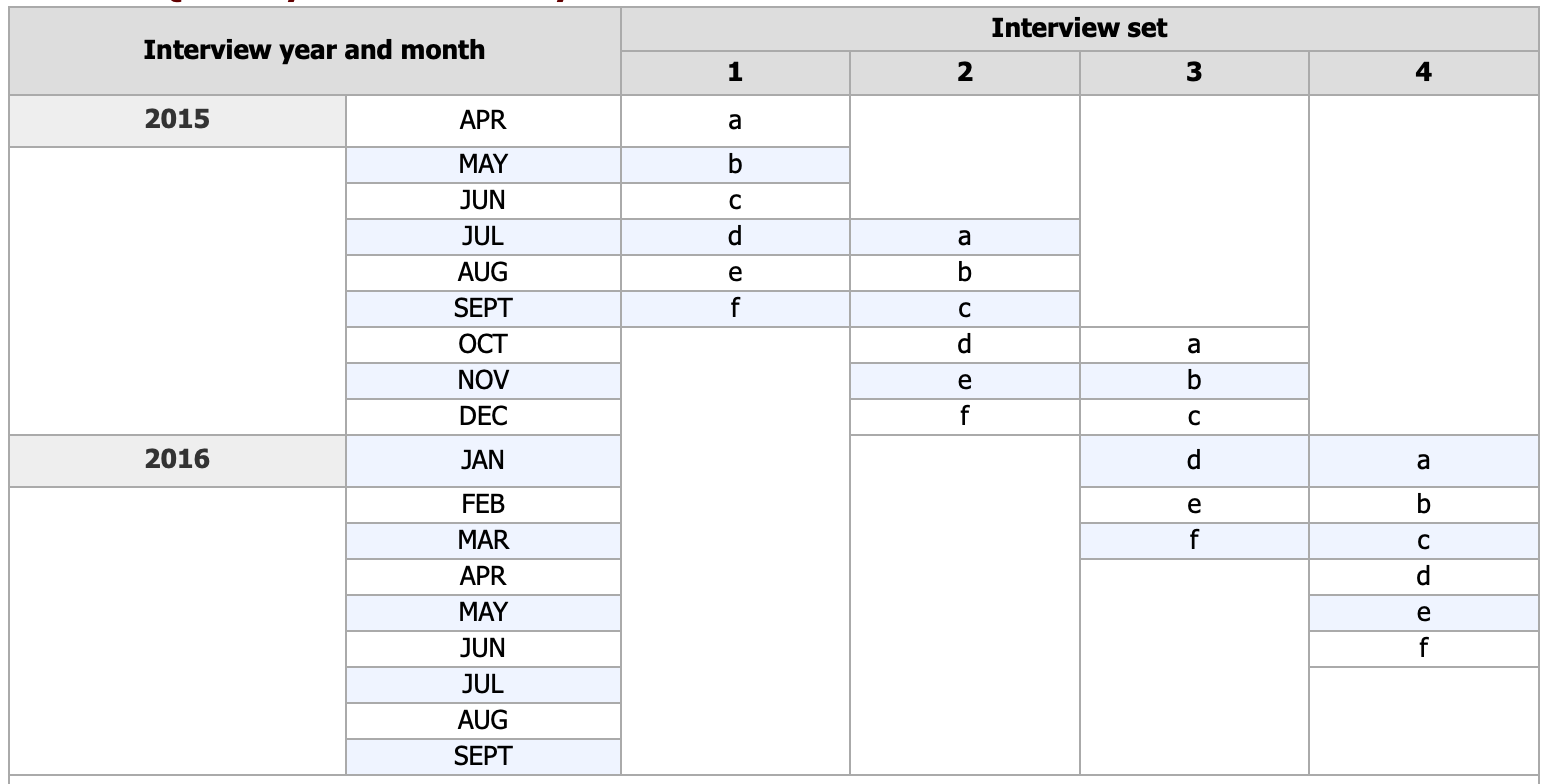
\includegraphics[width=.9\linewidth]{figures/CEX_rotation_table.png}
    \fnote{Columns show number of interview and a letter signals a specific household. Source: \url{https://www.bls.gov/opub/hom/cex/data.htm}}
    \label{fig:cex_rotation}
\end{figure}
%%%%%
It is important to highlight the limitations set by the usage of CEX data. As mentioned, the main objective of the CEX is to assess what goods the average household consumes to create the goods basket for inflation measurements. This focus results in a lack of interest in a dense documentation of household characteristics. For example, financial variables such as liquidity are only asked for in the initial screening interview, which for example prevents us form demeaning all controls in a panel like setting. Instead we have to rely on the inclusion of individual level fixed effects, which we explain in more detail in section \ref{sec:methodology}. While this is a disadvantage in comparison with other data sources, the CEX's richness in information on consumption behavior is unmatched. Keeping in mind the risk of measurement error through the self-reported consumption measurement, the CEX enables us to analyse not only the MPC for overall consumption but to dissect it and see which goods drive responses and heterogeneity seen in higher level estimates.